\documentclass[a4paper,11pt]{report}

\usepackage{a4wide}
\usepackage[english]{babel}
\usepackage{graphicx,subfigure}
\usepackage[pdftex,pdfauthor={Cedric~Cuypers, Kenzo~Tomita, Guy~Van~den~Broeck},pdftitle={Security Requirements: Poker Application}]{hyperref}
\usepackage[all]{hypcap}

\setcounter{secnumdepth}{3} 
\setlength{\parindent}{0pt} \setlength{\parskip}{1ex plus 0.5ex minus 0.2ex}


\author{Cedric~Cuypers, Kenzo~Tomita, Guy~Van~den~Broeck} 
% define title
\title{Security Requirements: Poker Application} 

\bibliographystyle{alpha}

\begin{document} 
% generates the title 
\maketitle 
% insert the table of contents 
\tableofcontents 

\chapter{Introduction}
This document starts from an existing architecture of a poker application that was originally designed with only an intuitive idea of security threats for poker applications. By modelling the data flow through the application we try to locate areas that can be subjected to these threats. 

For a subset of entities we apply STRIDE to elicit security threats and we use threat tree patterns to render these threats more concrete. The results are documented as misuse cases.

Finally, we present examples of business threats that cannot be discovered using the STRIDE methodology. 


\chapter{Identifying threats}
\section{DFDs}
Figure \ref{fig:context} shows the context level of the DFD. Figure \ref{fig:level_0} shows the level-0 DFD. The arrows are not annotated to make the diagram readable. A simplified version with only the player and annotated arrows can be found in figure \ref{fig:level_0_player}. In the following analysis only the interaction with the player will be considered as misuse cases, as those with an administrator as external entity are similar. Although some processes are complex and should be drilled down, we've chosen to do the STRIDE analysis on level-0 because it would already generate sufficient documentation.

There are several trust boundaries that can be identified in the DFDs. First of all there is the trust boundary between the external entities and the processes. All input coming from the external entities should be validated and the data flow from the processes to the external entities should be analyzed for not leaking sensitive, private or confidential data. Inside this trust boundary several smaller trust boundaries can be recognized. These are the processes that deal with sensitive, private data: 
\begin{itemize}
\item \textbf{Account Management:} account data should be protected and all data flowing out of this process should be verified extensively. 
\item \textbf{Table:} hole cards are confidential data only accessible for the player to whom they belong and the game engine to verify the winner at the end of a deal.
\item \textbf{Logging Engine:} the logging should happen in a secure way so there is no possibility to alter the log, therefor the log entries arriving at the logging engine should be validated. The log also contains very sensitive data, so the access is only allowed to a very limited number of entities and processes.
\end{itemize}
 

\begin{figure}[h]
  \begin{center}
    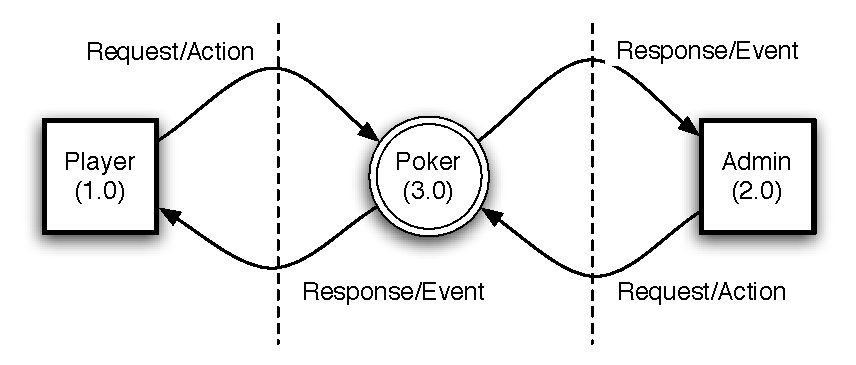
\includegraphics[scale=0.8]{context_diagram}
  \end{center}
  \caption{Context Level DFD}\label{fig:context}
\end{figure}

\begin{figure}[p]
  \begin{center}
    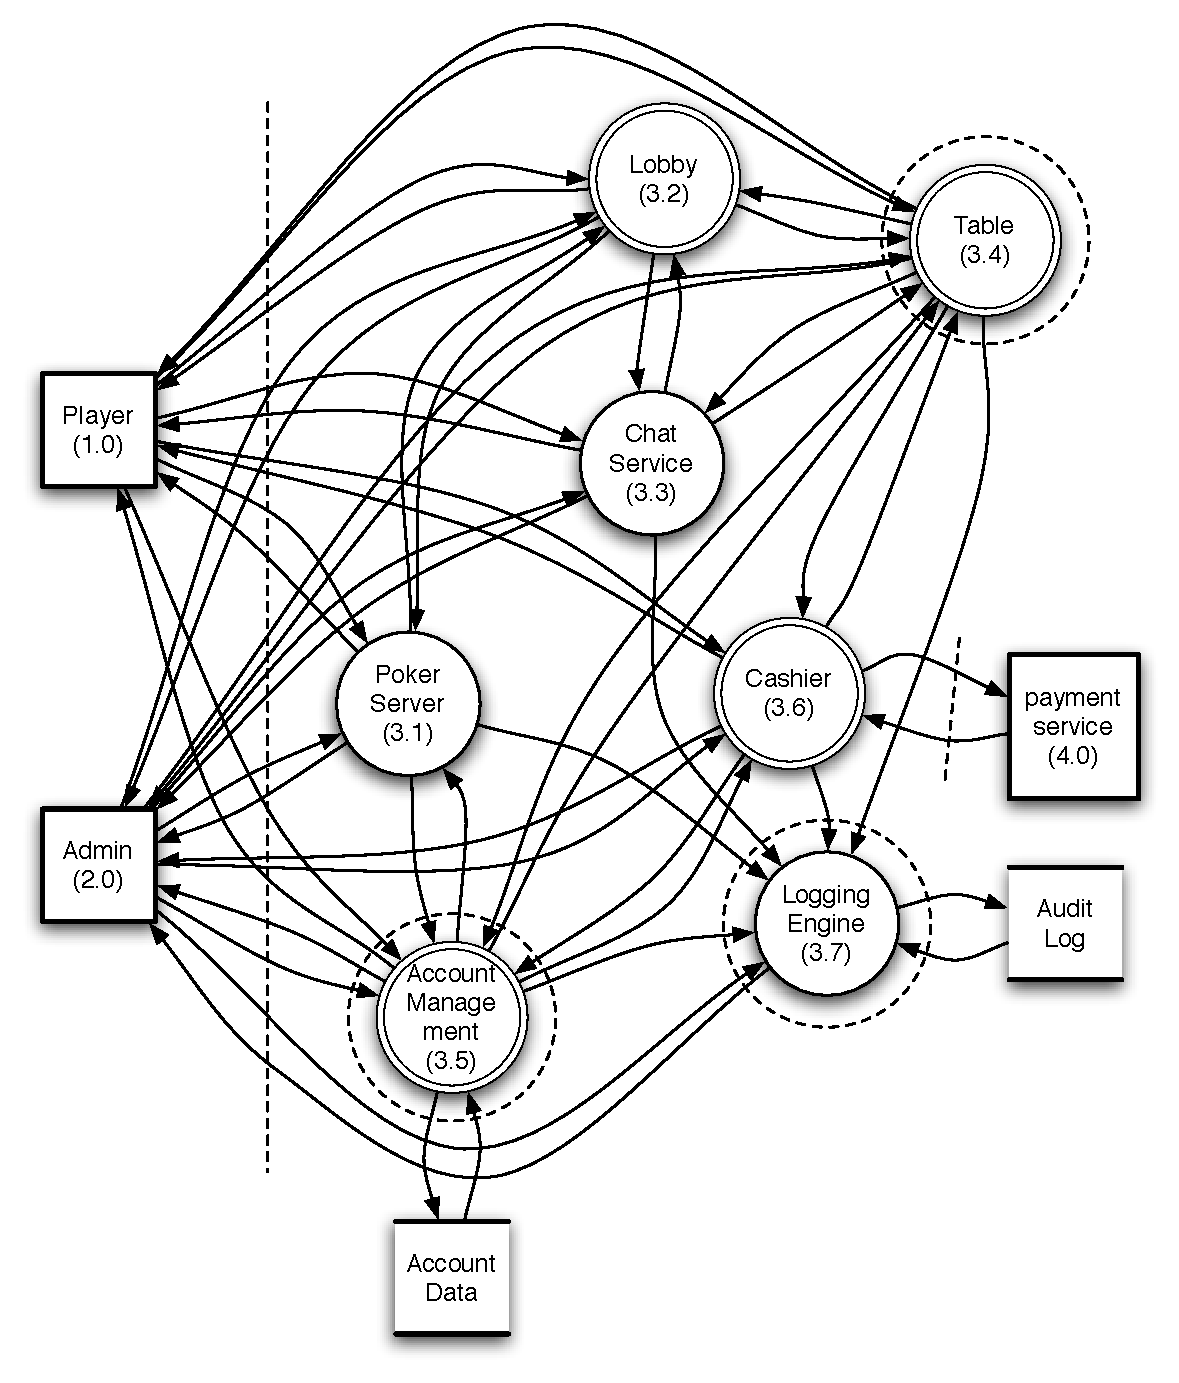
\includegraphics[scale=0.8]{dfd_level_0}
  \end{center}
  \caption{DFD Level-0}\label{fig:level_0}
\end{figure}

\begin{figure}[p]
  \begin{center}
    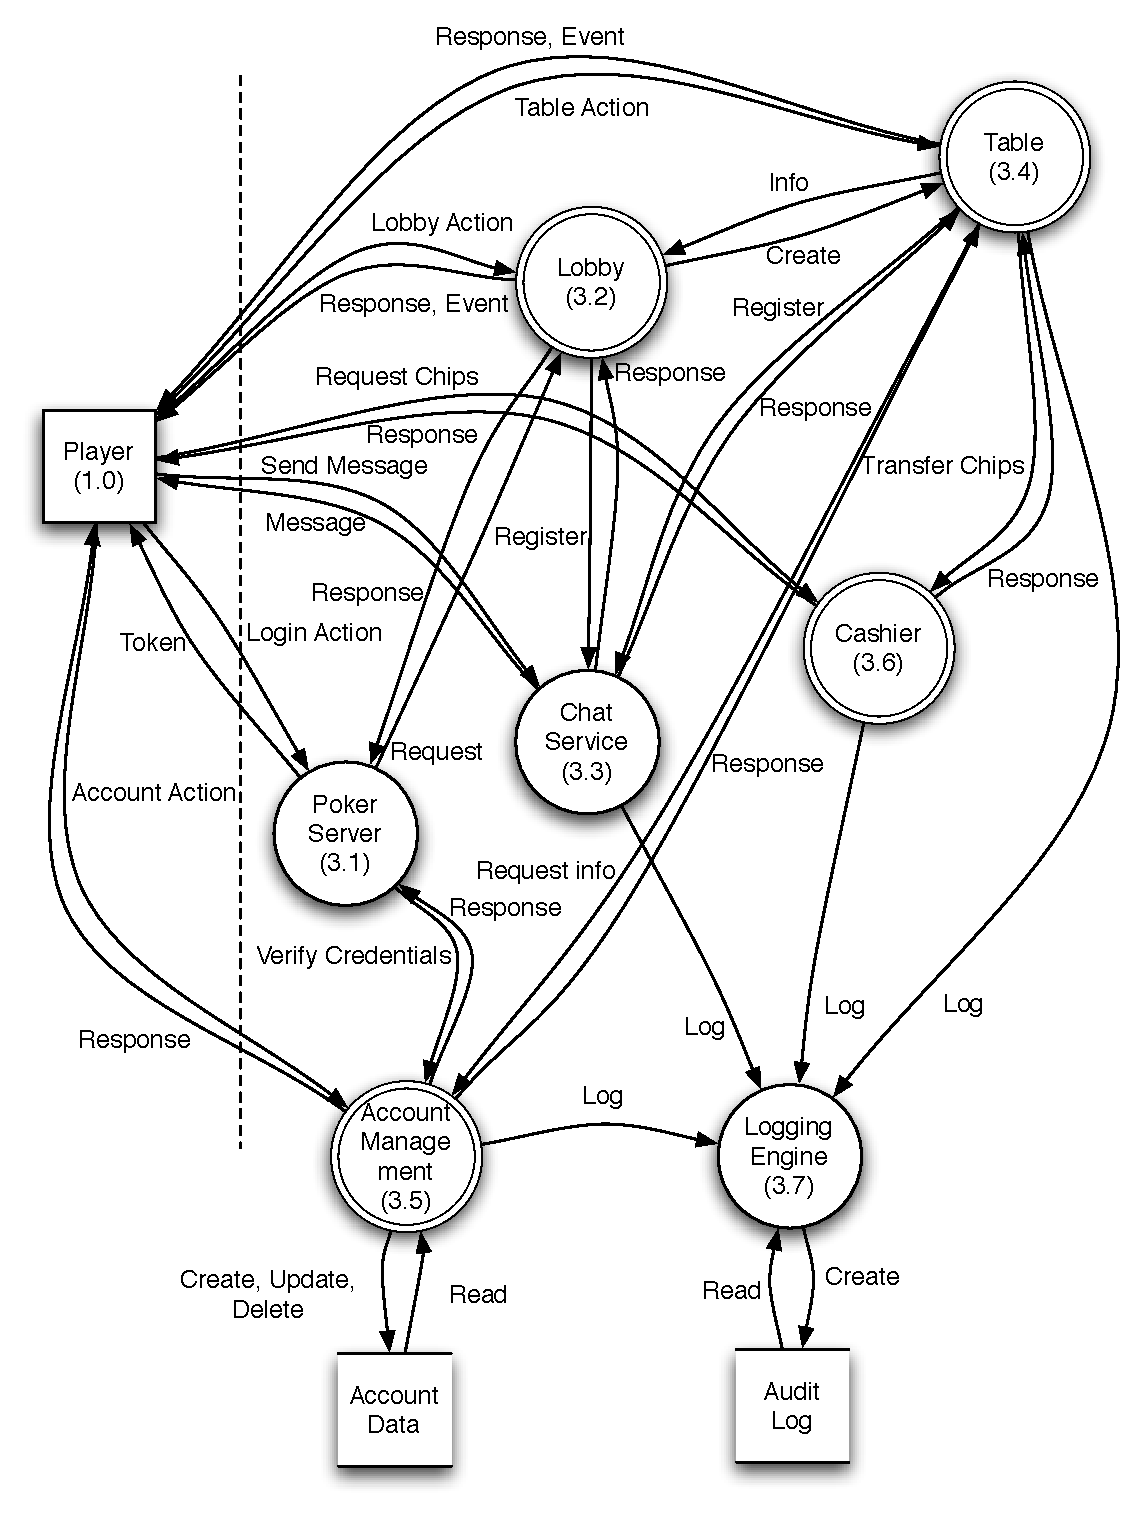
\includegraphics[scale=0.7]{dfd_level_0_player}
  \end{center}
  \caption{DFD Level-0 - only player}\label{fig:level_0_player}
\end{figure}

\section{Rationale}
\subsection{Assumptions}
\begin{itemize}
\item There is an internal policy to restrict physical access to the servers. 
\item There is no protection needed against an administrator with a debugger (can read and alter memory).
\item Side channels aren't available to mis-actors.
\item Data flow from a process to a data store is in our case always local and not subject to threats.
\end{itemize}

\section{Mapping STRIDE to DFD elements}

Taking the elements in figure \ref{fig:level_0} and mapping the STRIDE threats to tem results in the following table. The external entities \textit{Admin} and \textit{Payment Service} are subject to a number of threats that we chose not to go in to. Data flows from and to these entities are also not considered here. Similarly, data flows from and to the data stores are omitted.

\vspace{0.3cm}
\begin{center}
\begin{tabular}{| c || c || c | c | c | c | c | c |}
  \hline
  \textbf{DFD Element} 	& \textbf{Section}		& \textbf{S} 	& \textbf{T} 	& \textbf{R} 	& \textbf{I} 	& \textbf{D} 	& \textbf{E}	\\\hline
  \hline
  Player 		& \ref{PlayerCases}		& \ref{PlayerCasesS} 	& 	& \ref{PlayerCasesR} 		&  		&  		& 		\\\hline
  Admin 		& /			& / 		& 		& / 		&  		&  		& 		\\\hline
  Payment Service 	& /			& / 		& 		& / 		&  		&  		& 		\\\hline
  \hline
  Poker Server 		& \ref{PokerServerCases}	& \ref{PokerServerCasesS} 	& \ref{PokerServerCasesT}	& \ref{PokerServerCasesR} 	& \ref{PokerServerCasesI} 	& \ref{PokerServerCasesD} 	& \ref{PokerServerCasesE}	\\\hline
  Lobby 		& \ref{LobbyCases}		& \ref{LobbyCasesS} 	& \ref{LobbyCasesT}	& \ref{LobbyCasesR} 	& \ref{LobbyCasesI} 	& \ref{LobbyCasesD} 	& \ref{LobbyCasesE}	\\\hline
  Table 		& \ref{TableCases}		& \ref{TableCasesS} 	& \ref{TableCasesT}	& \ref{TableCasesR} 	& \ref{TableCasesI} 	& \ref{TableCasesD} 	& \ref{TableCasesE}	\\\hline
  Account Management 	& \ref{AccountManagementCases} 	& \ref{AccountManagementCasesS} 	& \ref{AccountManagementCasesT}	& \ref{AccountManagementCasesR} 	& \ref{AccountManagementCasesI} 	& \ref{AccountManagementCasesD} 	& \ref{AccountManagementCasesE}	\\\hline
  Logging Engine 	& \ref{LoggingEngineCases}	& \ref{LoggingEngineCasesS} 	& \ref{LoggingEngineCasesT}	& \ref{LoggingEngineCasesR} 	& \ref{LoggingEngineCasesI} 	& \ref{LoggingEngineCasesD} 	& \ref{LoggingEngineCasesE}	\\\hline
  Chat Service 		& /			& / 	& /	& / 	& / 	& / 	& /	\\\hline
  Cashier 		& /			& / 	& /	& / 	& / 	& / 	& /	\\\hline
  \hline
  Audit Log 		& \ref{AuditLogCases}		& 	& \ref{AuditLogCasesT}	& \ref{AuditLogCasesR} 	& \ref{AuditLogCasesI} 	& \ref{AuditLogCasesD}	& 	\\\hline
  Account Data 		& \ref{AccountDataCases}	& 	& \ref{AccountDataCasesT}	&  	& \ref{AccountDataCasesI} 	& \ref{AccountDataCasesD}	& 	\\\hline
  \hline
  Player $\leftrightarrow$ 
  Poker Server 		& \ref{PlayerFlowCases}		&	& \ref{PlayerFlowCasesT1}	&	& \ref{PlayerFlowCasesI1}	& \ref{PlayerFlowCasesD1}	&\\
  $\vdots$		& 				&	& \ref{PlayerFlowCasesT2}	&	& \ref{PlayerFlowCasesI2}	& \ref{PlayerFlowCasesD2}	&	\\
  			&				&	& \ref{PlayerFlowCasesT3}	&	& \ref{PlayerFlowCasesI3}	& \ref{PlayerFlowCasesD3}	\\
  			&				&	& \ref{PlayerFlowCasesT4}	&	& \ref{PlayerFlowCasesI4}	& \ref{PlayerFlowCasesD4}	\\\hline
  Table $\leftrightarrow$ 
  Logging Engine 	& \ref{LoggingEngineFlowCases}	&	& \ref{LoggingEngineFlowCasesT}	&	& \ref{LoggingEngineFlowCasesI}	& \ref{LoggingEngineFlowCasesD}	&	\\
  $\vdots$		& 				&	& 	&	& 	& 	&	\\\hline
\end{tabular}\end{center}
\vspace{0.3cm}

For the remaining data flows we chose to analyse them as a set of 4 different abstractions. Section \ref{PlayerFlowCases} goes in to more detail.

Furthermore, the processes \textit{Chat Service} and \textit{Cashier} are not elaborated on because they are more independent of other processes and functionality.

\section{Architecture based Misuse Cases}
\label{MisUseCases}

The misuse cases are ordered by the entity under threat. Repudiation is an important threat with legal consequences. Information disclosure is also important because it makes cheating very easy. Denial of Service attacks are less profitable for crooks and therefore less likely.

Threats that are located more to the exterior of te system (closer to the Player) are more likely to be feasible and are more important. For this reason we completely specified the threats for the Player and Poker Server. Because there are many data flows we chose to completely specify the threats for the different abstractions in section \ref{PlayerFlowCases} and \ref{LoggingEngineFlowCases}. Between the 2 data stores we chose to go in to detail for the account data.

\subsection{Player}
\label{PlayerCases}
\subsubsection{Spoofing a Player}
\label{PlayerCasesS}
\textbf{Summary:} \\
The mis-actor gains access to the poker server pretending to be a legitimate user. To achieve this goal he can use false credentials or credentials of an existing user. He could also bypass the authentication system to realize the same objective. \\
\textbf{Primary mis-actor:}
\begin{itemize}
\item Crook
\end{itemize}
\textbf{Basic path:}
\begin{itemize}
\item The mis-actor obtains the credentials of a legitimate player.
\item The mis-actor authenticates with the poker server.
\item The mis-actor can take actions on behalf of a legitimate player.
\end{itemize}
\textbf{Alternative paths:}
\begin{itemize}
\item The mis-actor bypasses the authentication system by exploiting a weakness.
\item The mis-actor finds a way to fake credentials.
\end{itemize}
\textbf{Capture points:}
\begin{itemize}
\item \textbf{Prevention:}
\begin{itemize}
\item Make sure credentials are well protected on the server side.
\item Transmit credentials over the wire securely.
\item Test credentials for uniqueness and complexity.
\item Certify client software to enforce that credentials are handled securely.
\end{itemize}
\end{itemize}
\textbf{Triggers:}\\
Always true, i.e., this can happen at any time. \\
\textbf{Preconditions:}
\begin{itemize}
\item Credentials can be falsified.
\item Credentials are not well protected.
\item There is no authentication system or the authentication system is too weak.
\end{itemize}
\textbf{Assumptions:}
\begin{itemize}
\item The players are careless with their credentials (e.g. store user name/password in a text file).
\item The players choose easy passwords.
\end{itemize}
\textbf{Worst case threat:}\\
The crook can play with the spoofed identity against his own identity and win all chips from spoofed identity. \\
\textbf{Prevention Guarantee:} \\
Only authentic users can gain access at the poker server. \\
\textbf{Stakeholders and risks:}
\begin{itemize}
\item Player: 
\begin{itemize}
\item Potential loss of money if his identity is misused and all chips are transfered to an other account.
\end{itemize}
\item Online Casino: 
\begin{itemize}
\item Lost confidence if security problems get publicized.
\end{itemize}
\end{itemize}

\subsubsection{Repudiation of a Player}
\label{PlayerCasesR}
\label{Repudiation of a Player}
\textbf{Primary mis-actor:}
\begin{itemize}
\item Crook
\end{itemize}
\textbf{Basic path:}
\begin{itemize}
\item The mis-actor performs an action or transaction.
\item The mis-actor repudiates the action or transaction For example, he repudiates his bet when it turns out that another player has a better hand.
\item The system fails to prove that the mis-actor is responsible.
\end{itemize}
\textbf{Alternative paths:}
\begin{itemize}
\item The mis-actor tampers with the logging process to remove evidence.
\end{itemize}
\textbf{Capture points:}
\begin{itemize}
\item \textbf{Prevention:}
\begin{itemize}
\item Use a strong signature system for messages originating from the player.
\item Use antireplay defences.
\item Log all actions and transactions.
\item Secure access to the logging process.
\end{itemize}
\end{itemize}

\subsection{Poker Server}
\label{PokerServerCases}
\subsubsection{Spoofing the poker server}
\label{PokerServerCasesS}
\textbf{Primary mis-actor:}
\begin{itemize}
\item Crook
\end{itemize}
\textbf{Basic path:}
\begin{itemize}
\item The mis-actor prepares the process that can spoof a poker server.
\item The mis-actor deploys its process on the online casino servers (performed by a skilled insider).
\item The mis-actor can cheat and steal sensitive data from the users.
\end{itemize}
\textbf{Alternative paths:}
\begin{itemize}
\item The mis-actor deploys its process on an external server (performed by a skilled outsider).
\end{itemize}
\textbf{Capture points:}
\begin{itemize}
\item \textbf{Prevention:}
\begin{itemize}
\item Only administrators of the online casino can place code on the online poker servers.
\item Only the code that is running on trusted locations can be used as part of the system.
\item Poker servers are authenticated.
\item Messages coming out of the poker server are signed.
\end{itemize}
\end{itemize}

\subsubsection{Tampering with the poker server}
\label{PokerServerCasesT}
\textbf{Primary mis-actor:}
\begin{itemize}
\item Crook
\end{itemize}
\textbf{Basic path:}
\begin{itemize}
\item The mis-actor sends invalid input to the poker server.
\item The message corrupts the state of the poker server. 
\item While the poker server is in the corrupted state, the mis-actor controls the behavior of that poker server.
\item The mis-actor can cheat and steal sensitive data from the users.
\end{itemize}
\textbf{Alternative paths:}
\begin{itemize}
\item The mis-actor provides false credentials (spoofing an administrator) and modifies the poker server.
\end{itemize}
\textbf{Capture points:}
\begin{itemize}
\item \textbf{Prevention:}
\begin{itemize}
\item All input is validated.
\item Spoofing an administrator should be impossible.
\end{itemize}
\end{itemize}

\subsubsection{Repudiation of the poker server}
\label{PokerServerCasesR}
\textbf{Primary mis-actor:}
\begin{itemize}
\item Crook
\end{itemize}
\textbf{Basic path:}
\begin{itemize}
\item The mis-actor gains access to the poker server.
\item The mis-actor sends back a response to the player that is misleading.
\item The mis-actor repudiates having sent the response in question.
\item The player fails to prove that the server/mis-actor is responsible.
\end{itemize}
\textbf{Alternative paths:}
\begin{itemize}
\item The mis-actor tampers with the logging process to remove evidence.
\end{itemize}
\textbf{Capture points:}
\begin{itemize}
\item \textbf{Prevention:}
\begin{itemize}
\item Use a strong signature system for messages sent to the player.
\item Use antireplay defences.
\item Log all actions and transactions.
\item Secure access to the logging process
\end{itemize}
\end{itemize}

\subsubsection{Information disclosure at the poker server}
\label{PokerServerCasesI}
\textbf{Primary mis-actor:}
\begin{itemize}
\item Crook
\end{itemize}
\textbf{Basic path:}
\begin{itemize}
\item The mis-actor spoofs another actor with access to private information (e.g. user names, passwords, ...).
\item The mis-actor uses the private information.
\end{itemize}
\textbf{Alternative paths:}
\begin{itemize}
\item Elevation of privilege of the mis-actor leads to information disclosure.
\item The mis-actor sends invalid input to the poker server.
\item The mis-actor has access to the memory and can alter its state (e.g. debugging mode).
\end{itemize}
\textbf{Capture points:}
\begin{itemize}
\item \textbf{Prevention:}
\begin{itemize}
\item All input is validated.
\end{itemize}
\end{itemize}

\subsubsection{DoS against the poker server}
\label{PokerServerCasesD}
\textbf{Primary mis-actor:}
\begin{itemize}
\item Crook
\end{itemize}
\textbf{Basic path:}
\begin{itemize}
\item The mis-actor sends invalid input to the poker server. 
\item The poker server crashes.
\item The poker server becomes unavailable.
\end{itemize}
\textbf{Alternative paths:}
\begin{itemize}
\item The mis-actor crashes the poker server by tampering with the poker server.
\item The mis-actor consumes application-specific resources (e.g. send more login requests per second than the poker server can handle).
\item The mis-actor consumes fundamental resources.
\end{itemize}
\textbf{Capture points:}
\begin{itemize}
\item \textbf{Prevention:}
\begin{itemize}
\item All input is validated.
\item The poker server is load-balanced.
\end{itemize}
\item \textbf{Detection:}
\begin{itemize}
\item Access to the poker server is securely logged.
\end{itemize}
\end{itemize}

\subsubsection{Elevation of privilege at the poker server}
\label{PokerServerCasesE}
\textbf{Primary mis-actor:}
\begin{itemize}
\item Crook
\end{itemize}
\textbf{Basic path:}
\begin{itemize}
\item The mis-actor logs in.
\item He activates the role (administrator) with higher privileges.
\item The mis-actor gains higher privileges. 
\item The mis-actor misuses the higher privileges.
\end{itemize}
\textbf{Alternative paths:}
\begin{itemize}
\item The mis-actor spoofs the identity of an other actor (administrator) with higher privileges.
\item The mis-actor tampers with the poker server to gain more privileges. 
\item The mis-actor sends invalid input to the poker server. 
\item The mis-actor has access to the memory and can alter its state (e.g. debugging mode).
\end{itemize}
\textbf{Capture points:}
\begin{itemize}
\item \textbf{Prevention:}
\begin{itemize}
\item Authentication and authorisation system that verifies credentials.
\item Spoofing user and tampering with poker server prevention.
\end{itemize}
\item \textbf{Detection:}
\begin{itemize}
\item Access to the poker server is securely logged. The log can be compared with the security policy to verify if an actor is allowed to do the action.
\end{itemize}
\end{itemize}

\subsection{Lobby}
\label{LobbyCases}
\subsubsection{Spoofing a lobby}
\label{LobbyCasesS}
\textbf{Summary:} \\
The mis-actor prepares a process to spoof the lobby and deploys it on one of the online casino servers or on an external server. Every player connecting to a table through the lobby can be diverted to an untrusted table.
\subsubsection{Tampering with the lobby}
\label{LobbyCasesT}
\textbf{Summary:} \\
The mis-actor tampers with the lobby to modify its functionality. A player connecting to a table through the lobby can be diverted to an untrusted table. 
\subsubsection{Repudiation of an action at the lobby}
\label{LobbyCasesR}
\textbf{Summary:} \\
The lobby can deny access to a table for a certain user and deny having done so.

\subsubsection{Information disclosure at the lobby}
\label{LobbyCasesI}
\textbf{Summary:} \\
The mis-actor can obtain private information through spoofing or tampering with the lobby process. He could see private tables or tournament settings.

\subsubsection{DoS against the lobby}
\label{LobbyCasesD}
\textbf{Summary:} \\
The mis-actor performs actions leading to a crash or overloading the capacity of the lobby. As a result, the lobby can no longer be reached by the users.
\subsubsection{Elevation of privilege at the lobby}
\label{LobbyCasesE}
\textbf{Summary:} \\
The mis-actor performs actions leading to the possibility to do administrator actions. He can achieve this by presenting false credentials, spoofing an administrator or tampering with the lobby or account management.

\subsection{Table}\
\label{TableCases}
\subsubsection{Spoofing a table}
\label{TableCasesS}
\textbf{Summary:} \\
The mis-actor prepares a process to spoof the table and deploys it on one of the online casino servers or on an external server. Every player connecting to this table can be scammed. The spoofed table could provide the mis-actor with all confidential information or deal crafted hands to maximize the profit of the mis-actor (e.g. deal a full house to an innocent player and deal a four of a kind to himself and lure the innocent player to go all-in).
\subsubsection{Tampering with a table}
\label{TableCasesT}
\textbf{Summary:} \\
The mis-actor tampers with the lobby to modify its functionality. Every player connecting to this table can be scammed. The tampered table could provide the mis-actor with all confidential information or deal crafted hands to maximize the profit of the mis-actor (e.g. deal a full house to an innocent player and deal a four of a kind to himself and lure the innocent player to go all-in).
\subsubsection{Repudiation of an action at a table}
\label{TableCasesR}
\textbf{Summary:} \\
The online casino denies a player has won a number of chips or has received certain hole cards. This is possible if there is no log or if the log could be modified. It is also possible that the hand evaluation system has been tampered and this should be detected afterwards. 
\subsubsection{Information disclosure at a table}
\label{TableCasesI}
\textbf{Primary mis-actor:}
\begin{itemize}
\item Crook
\end{itemize}
\textbf{Basic path:}
\begin{itemize}
\item The mis-actor spoofs an other actor with access to private information regarding this table
(e.g. pocket cards of players, ...).
\item The mis-actor uses the private information.
\end{itemize}
\textbf{Alternative paths:}
\begin{itemize}
\item Elevation of privilege of the mis-actor leads to information disclosure.
\item The mis-actor sends invalid input to the table.
\item The mis-actor has access to the memory and can alter its state (e.g. debugging mode).
\end{itemize}
\textbf{Capture points:}
\begin{itemize}
\item \textbf{Prevention:}
\begin{itemize}
\item All input is validated.
\end{itemize}
\item \textbf{Detection:}
\begin{itemize}
\item The behavior of the mis-actor is influenced by the information disclosure. This altered behavior could be detected by examining the logs.
\end{itemize}
\end{itemize}

\subsubsection{DoS against a table}
\label{TableCasesD}
\textbf{Summary:} \\
The mis-actor performs actions leading to a crash or overloading the capacity of the table. As a result, the table can no longer be reached by the users.

\subsubsection{Elevation of Privilege at the table}
\label{TableCasesE}
\textbf{Summary:} \\
The mis-actor performs actions leading to the possibility to do administrator actions. He can achieve this by presenting false credentials, spoofing an administrator or tampering with the lobby or account management.

\subsection{Account Management}
\label{AccountManagementCases}

\subsubsection{Spoofing the account management system}
\label{AccountManagementCasesS}
\textbf{Summary:} \\
The mis-actor gains access to the account management system or manages to pretend he is the account management system by obtaining or falsifying credentials. By doing so the mis-actor has control over how incoming requests and data are processed. He can for instance trick other processes in to accepting bad credentials for authentication.

\subsubsection{Tampering with the account management system}
\label{AccountManagementCasesT}
\textbf{Summary:} \\
The mis-actor can tamper with the account management system to always accept credentials for a certain fake user.

\subsubsection{Repudiation of using the account management system}
\label{AccountManagementCasesR}
\textbf{Summary:} \\
The casino can deny access to a user in critical moments and deny having done so. When a user changes his credit card number or other personal information the account management system can deny having received that request. When a payment fails afterwards the user cannot seek compensation from the casino.

\subsubsection{Information disclosure of the account management system}
\label{AccountManagementCasesI}
\textbf{Summary:} \\
When the mis-actor corrupts te account management system he can obtain private information such as passwords and credit card numbers. This can be done by through spoofing or tampering with the process.

\subsubsection{DoS against the account management system}
\label{AccountManagementCasesD}
\textbf{Summary:} \\
By sending bad input to the account management system or by sending many requests at once, the mis-user can overload the process. This can result in legitimate users not being able to authenticate with the system or change their account data.

\subsubsection{Elevation of Privilege at the account management system}
\label{AccountManagementCasesE}
\textbf{Summary:} \\
Through spoofing, tampering or exploiting the authorization system, the mis-actor can obtain admin privileges. In the account management system he will be able to e.g. kick or ban opponents.

\subsection{Logging Engine}
\label{LoggingEngineCases}

\subsubsection{Spoofing the logging engine}
\label{LoggingEngineCasesS}
\textbf{Summary:} \\
The mis-actor gains access to the logging engine or manages to pretend to be the logging engine by obtaining or falsifying credentials. This way he can stop logging messages from being made persistent by the real logging engine.

\subsubsection{Tampering with the logging engine}
\label{LoggingEngineCasesT}
\textbf{Summary:} \\
The mis-actor can tamper with the logging engine and send different data to the audit log than was received from other processes. Alternatively, he can send logging data to the audit log that is made up.

\subsubsection{Repudiation of using the logging engine}
\label{LoggingEngineCasesR}
\textbf{Summary:} \\
The logging engine can deny having recieved logging data that didn't make it to the physical audit log. The casino can deny that certain audit data was sent from the logging engine and is valid.

\subsubsection{Information disclosure of the logging engine}
\label{LoggingEngineCasesI}
\textbf{Summary:} \\
The mis-actor can obtain private information through spoofing or tampering with the logging process. This way he could e.g. see the hidden cards of an opponent.

\subsubsection{DoS against the logging engine}
\label{LoggingEngineCasesD}
\textbf{Summary:} \\
By sending bad data to the logging engine or by sending many requests at once, the mis-user can overload the process. This can result in valid logging data being lost by the process because it can't store the incoming information.

\subsubsection{Elevation of Privilege at the logging engine}
\label{LoggingEngineCasesE}
\textbf{Summary:} \\
Through spoofing, tampering or exploiting the authorization system, the mis-actor can obtain admin privileges. AS a result he can, for instance, shut down logging.

\subsection{Audit Log}
\label{AuditLogCases}

\subsubsection{Tampering with the audit log}
\label{AuditLogCasesT}
\textbf{Summary:} \\
The misuser can tamper with the audit log when he bypasses the protection or monitor, or when he exploits overcapacity failures. The logging data can then be modified or erased.

\subsubsection{Repudiation of logging something in the audit log}
\label{AuditLogCasesR}
\textbf{Summary:} \\
The mis-actor can modify or obscure data in the audit log to 

\subsubsection{Information disclosure of the audit log}
\label{AuditLogCasesI}
\textbf{Summary:} \\
When the mis-actor bypasses te protection scheme and the data is weakly encrypted he might be able to obtain logging information. This can e.g be credit card information, transaction information or private cards. Information leakage can also occur when removed data isn't cleared correctly from the data store or when te mis-actor spoofs an entity that has access to the data store.

\subsubsection{DoS against the audit log}
\label{AuditLogCasesD}
\textbf{Summary:} \\
By sending bad data to the audit log (SQL injecton) or by sending many requests at once, the mis-user can overload the data store. This can result in valid logging data being lost because the data store has e.g. run out of memory or disk space.

\subsection{Account Data}
\label{AccountDataCases}

\subsubsection{Tampering with account data}
\label{AccountDataCasesT}
\textbf{Primary mis-actor:}
\begin{itemize}
\item Crook
\end{itemize}
\textbf{Basic path:}
\begin{itemize}
\item The mis-actor gains access to the data store
\item The mis-actor puts data directly in the data store
\end{itemize}
\textbf{Alternative paths:}
\begin{itemize}
\item The mis-actor removes data directly from the data store
\item There may be overcapacity failures: the mis-actor floods the data store by placing large 
amounts of data into the data store. As a consequence data in the beginning of the store might be overwritten
, data written to the store might be discarded or the data store might crash, depending on the implementation of
the data store.
\end{itemize}
\textbf{Capture points:}
\begin{itemize}
\item \textbf{Prevention:}
\begin{itemize}
\item placing and removing of data in the data store is securely logged
\item data store is protected by the internal policies
\item extra-monitor access is impossible (behind a reliable firewall)
\item overcapacity failures are handled accordingly
\item only private or local networks are used for communication between the account management process 
and the account data store.
\end{itemize}
\item \textbf{Detection:}
\begin{itemize}
\item logs can be searched for adding of removing falsified data
\end{itemize}
\end{itemize}

\subsubsection{Information disclosure of account data}
\label{AccountDataCasesI}
\textbf{Primary mis-actor:}
\begin{itemize}
\item Crook
\end{itemize}
\textbf{Basic path:}
\begin{itemize}
\item The mis-actor gains access to the data store.
\item The mis-actor reads private data from data store.
\end{itemize}
\textbf{Alternative paths:}
\begin{itemize}
\item The mis-actor spoofs the account management process
\end{itemize}
\textbf{Capture points:}
\begin{itemize}
\item \textbf{Prevention:}
\begin{itemize}
\item encrypting the data 
\item data store is protected by the internal policies
\item extra-monitor access is impossible (behind a reliable firewall)
\item only private or local networks are used for communication between the account management process 
and the account data store.
\item prevent spoofing of account management process
\end{itemize}
\end{itemize}

\subsubsection{DoS against account data}
\label{AccountDataCasesD}
\textbf{Primary mis-actor:}
\begin{itemize}
\item Crook
\end{itemize}
\textbf{Basic path:}
\begin{itemize}
\item The mis-actor gains access to the data store.
\item The mis-actor corrupts the data store by sending invalid input.
\item The data store crashes and becomes unavailable.
\end{itemize}
\textbf{Alternative paths:}
\begin{itemize}
\item The mis-actor floods the data store by placing large amounts of data into the data store and exceeds the 
capacity of the data store.
\item The mis-actor consumes application-specific resources (e.g. submit more queries per second that the data 
store can handle).
\item The mis-actor injects malicious SQL queries (or other) to an user of the data store. When this injection reaches the data store it crashes.
\end{itemize}
\textbf{Capture points:}
\begin{itemize}
\item \textbf{Prevention:}
\begin{itemize}
\item Invalid queries are filtered.
\item Data store is protected by the internal policies.
\item Extra-monitor access is impossible (behind a reliable firewall).
\item Only private or local networks are used for communication between the account management process 
and the account data store.
\item The data store is load-balanced.
\end{itemize}
\end{itemize}

\subsection{Data Flows from a Player}
\label{PlayerFlowCases}

According to \cite[p117]{1202957}, one of the first concerns before doing threat analysis should be to reduce the number of entities to analyze.
Here we choose to reduce the number of data flows from/to the Player because interaction between a Player and the different processes is very similar (using the same technology, similar entities with similar confidentiality). We only consider requests for tokens (login actions), actions sent to a process, tokens sent to a Player and events/responses sent to a Player.

\subsubsection{Tampering with token requests}
\label{PlayerFlowCasesT1}
\textbf{Primary mis-actor:}
\begin{itemize}
\item Crook
\end{itemize}
\textbf{Basic path:}
\begin{itemize}
\item The mis-actor find a weakness in the integrity of token requests.
\item The mis-actor intercepts a token request sent by another Player.
\item The mis-actor replays the token request to obtain a token.
\end{itemize}
\textbf{Alternative paths:}
\begin{itemize}
\item The mis-actor spoofs another Player to send fake token requests.
\item The mis-actor performs a MITM attack and eavesdrop on the token requests sent by a genuine Player.
\end{itemize}
\textbf{Capture points:}
\begin{itemize}
\item \textbf{Prevention:}
\begin{itemize}
\item Use antireplay defences and a strong message and channel integrity algorithm.
\item Prevent spoofing of Players.
\end{itemize}
\end{itemize}

\subsubsection{Tampering with tokens}
\label{PlayerFlowCasesT2}
\textbf{Primary mis-actor:}
\begin{itemize}
\item Crook
\end{itemize}
\textbf{Basic path:}
\begin{itemize}
\item The mis-actor find a weakness in the integrity of tokens sent to the Player.
\item The mis-actor intercepts a token.
\item The mis-actor modifies token before sending it to the Player with a MITM attack. The modified token can refer to a process spoofed by the mis-actor..
\end{itemize}
\textbf{Alternative paths:}
\begin{itemize}
\item The mis-actor spoofs the Poker Server to send fake tokens.
\item The mis-actor modifies or replays tokens.
\end{itemize}
\textbf{Capture points:}
\begin{itemize}
\item \textbf{Prevention:}
\begin{itemize}
\item Use antireplay defences and a strong message and channel integrity algorithm.
\item Prevent spoofing of the Poker Server.
\end{itemize}
\end{itemize}

\subsubsection{Tampering with actions}
\label{PlayerFlowCasesT3}
\textbf{Primary mis-actor:}
\begin{itemize}
\item Crook
\end{itemize}
\textbf{Basic path:}
\begin{itemize}
\item The mis-actor find a weakness in the integrity of actions.
\item The mis-actor changes messages to his advantage, sends fake messages that go undetected or replays messages sent by a Player. For example, the mis-actor can replace the bet amount by a larger number when he has very good cards)
\end{itemize}
\textbf{Alternative paths:} 
\begin{itemize}
\item The mis-actor violates the integrity of the channel to tamper with the data flow.
\item The mis-actor spoofs a Player to send fake actions.
\end{itemize}
\textbf{Capture points:}
\begin{itemize}
\item \textbf{Prevention:}
\begin{itemize}
\item Use antireplay defences and a strong message and channel integrity algorithm.
\item Prevent spoofing of Players.
\end{itemize}
\end{itemize}

\subsubsection{Tampering with responses and events}
\label{PlayerFlowCasesT4}
\textbf{Primary mis-actor:}
\begin{itemize}
\item Crook
\end{itemize}
\textbf{Basic path:}
\begin{itemize}
\item The mis-actor find a weakness in the integrity of responses or events.
\item The mis-actor changes events to his advantage, sends fake events or replays events For example, the mis-actor can replace the pocket cards sent to another player by aces to trick him in to betting excessively.
\end{itemize}
\textbf{Alternative paths:}
\begin{itemize}
\item The mis-actor violates the integrity of the channel to tamper with the data flow.
\item The mis-actor spoofs the Poker Server to send fake actions.
\end{itemize}
\textbf{Capture points:}
\begin{itemize}
\item \textbf{Prevention:}
\begin{itemize}
\item Use antireplay defences and a strong message and channel integrity algorithm.
\item Prevent spoofing the Poker Server.
\end{itemize}
\end{itemize}


\subsubsection{Information Disclosure of token requests}
\label{PlayerFlowCasesI1}
\textbf{Primary mis-actor:}
\begin{itemize}
\item Crook
\end{itemize}
\textbf{Basic path:}
\begin{itemize}
\item The mis-actor finds a weakness in the confidentiality of token requests and the channel used to send them.
\item The mis-actor observes who is playing and what modules they are requesting tokens for.
\end{itemize}
\textbf{Alternative paths:}
\begin{itemize}
\item The mis-actor sets up a MITM attack.
\item The mis-actor observes data through a side channel.
\end{itemize}
\textbf{Capture points:}
\begin{itemize}
\item \textbf{Prevention:}
\begin{itemize}
\item Use stong message confidentiality.
\item Use strong channel confidentiality.
\item Review known side channel vulnerabilities to determine if they apply and fix them.
\end{itemize}
\end{itemize}

\subsubsection{Information Disclosure of tokens}
\label{PlayerFlowCasesI2}
\textbf{Primary mis-actor:}
\begin{itemize}
\item Crook
\end{itemize}
\textbf{Basic path:}
\begin{itemize}
\item The mis-actor finds a weakness in the confidentiality of token message and the channel used to send them.
\item The mis-actor observes the tokens and can use them in a spoofing attack.
\end{itemize}
\textbf{Alternative paths:}
\begin{itemize}
\item The mis-actor sets up a MITM attack.
\item The mis-actor observes data through a side channel.
\end{itemize}
\textbf{Capture points:}
\begin{itemize}
\item \textbf{Prevention:}
\begin{itemize}
\item Use stong message confidentiality.
\item Use strong channel confidentiality.
\item Review known side channel vulnerabilities to determine if they apply and fix them.
\end{itemize}
\end{itemize}

\subsubsection{Information Disclosure of actions}
\label{PlayerFlowCasesI3}
\textbf{Primary mis-actor:}
\begin{itemize}
\item Crook
\end{itemize}
\textbf{Basic path:}
\begin{itemize}
\item The mis-actor finds a weakness in the confidentiality of actions and the channel used to send them.
\item The mis-actor observes the actions and can abuse private chat information and other confidential actions performed by the Player.
\end{itemize}
\textbf{Alternative paths:}
\begin{itemize}
\item The mis-actor sets up a MITM attack.
\item The mis-actor observes data through a side channel.
\end{itemize}
\textbf{Capture points:}
\begin{itemize}
\item \textbf{Prevention:}
\begin{itemize}
\item Use stong message confidentiality.
\item Use strong channel confidentiality.
\item Review known side channel vulnerabilities to determine if they apply and fix them.
\end{itemize}
\end{itemize}

\subsubsection{Information Disclosure of responses and events}
\label{PlayerFlowCasesI4}
\textbf{Primary mis-actor:}
\begin{itemize}
\item Crook
\end{itemize}
\textbf{Basic path:}
\begin{itemize}
\item The mis-actor finds a weakness in the confidentiality of events/responses and the channel used to send them.
\item The mis-actor observes events that give him an unfair advantage in the game, like the pocket cards of competitors. 
\end{itemize}
\textbf{Alternative paths:}
\begin{itemize}
\item The mis-actor sets up a MITM attack.
\item The mis-actor observes data through a side channel.
\end{itemize}
\textbf{Capture points:}
\begin{itemize}
\item \textbf{Prevention:}
\begin{itemize}
\item Use stong message confidentiality.
\item Use strong channel confidentiality.
\item Review known side channel vulnerabilities to determine if they apply and fix them.
\end{itemize}
\end{itemize}


\subsubsection{Denial of Service of token requests}
\label{PlayerFlowCasesD1}
\textbf{Primary mis-actor:}
\begin{itemize}
\item Crook
\end{itemize}
\textbf{Basic path:}
\begin{itemize}
\item The mis-actor incapacitates the channel by incapacitating the Player or process.
\item The Player cannot request tokens.
\end{itemize}
\textbf{Alternative paths:}
\begin{itemize}
\item The mis-actor consumes resources required by the Player or process.
\item The mis-actor corrupts the token requests.
\item The mis-actor preplays token requests, making that functionality unavailable for a Player.
\end{itemize}
\textbf{Capture points:}
\begin{itemize}
\item \textbf{Prevention:}
\begin{itemize}
\item Prevent tampering, spoofing and DOS of the endpoints and data flow.
\item Limit the number of resources the process depends on.
\end{itemize}
\end{itemize}

\subsubsection{Denial of Service of tokens}
\label{PlayerFlowCasesD2}
\textbf{Primary mis-actor:}
\begin{itemize}
\item Crook
\end{itemize}
\textbf{Basic path:}
\begin{itemize}
\item The mis-actor incapacitates the channel by incapacitating the Player or process.
\item The Player cannot receive tokens.
\end{itemize}
\textbf{Alternative paths:}
\begin{itemize}
\item The mis-actor consumes resources required by the Player or process.
\end{itemize}
\textbf{Capture points:}
\begin{itemize}
\item \textbf{Prevention:}
\begin{itemize}
\item Prevent tampering, spoofing and DOS of the endpoints and data flow.
\item Limit the number of resources the process depends on.
\end{itemize}
\end{itemize}

\subsubsection{Denial of Service of actions}
\label{PlayerFlowCasesD3}
\textbf{Primary mis-actor:}
\begin{itemize}
\item Crook
\end{itemize}
\textbf{Basic path:}
\begin{itemize}
\item The mis-actor incapacitates the channel by incapacitating the Player or process.
\item The Player cannot perform actions. For example, this can lead to timeouts where the server folds on behalf of a non-responsive player, giving an unfair advantage to the mis-actor.
\end{itemize}
\textbf{Alternative paths:}
\begin{itemize}
\item The mis-actor consumes resources required by the Player or process.
\item The mis-actor corrupts the actions.
\item The mis-actor preplays actions, making them unavailable for a Player.
\end{itemize}
\textbf{Capture points:}
\begin{itemize}
\item \textbf{Prevention:}
\begin{itemize}
\item Prevent tampering, spoofing and DOS of the endpoints and data flow.
\item Limit the number of resources the process depends on.
\end{itemize}
\end{itemize}

\subsubsection{Denial of Service of responses and events}
\label{PlayerFlowCasesD4}
\textbf{Primary mis-actor:}
\begin{itemize}
\item Crook
\end{itemize}
\textbf{Basic path:}
\begin{itemize}
\item The mis-actor incapacitates the channel by incapacitating the Player or process.
\item The Player cannot receive events/responses.
\end{itemize}
\textbf{Alternative paths:}
\begin{itemize}
\item The mis-actor consumes resources required by the Player or process.
\end{itemize}
\textbf{Capture points:}
\begin{itemize}
\item \textbf{Prevention:}
\begin{itemize}
\item Prevent tampering, spoofing and DOS of the endpoints and data flow.
\item Limit the number of resources the process depends on.
\end{itemize}
\end{itemize}

\subsection{Data Flows to Logging Engine}
\label{LoggingEngineFlowCases}

\subsubsection{Tampering with logging requests}
\label{LoggingEngineFlowCasesT}
\textbf{Primary mis-actor:}
\begin{itemize}
\item Crook
\end{itemize}
\textbf{Basic path:}
\begin{itemize}
\item The mis-actor find a weakness in the integrity of logging requests.
\item The mis-actor intercepts a logging request sent by another process.
\item The mis-actor replays the logging request to duplicate the thing to be logged.
\end{itemize}
\textbf{Alternative paths:}
\begin{itemize}
\item The mis-actor spoofs another Player to send fake logging requests.
\item The mis-actor performs a MITM attack and eavesdrop on the logging requests sent by a genuine process.
\end{itemize}
\textbf{Capture points:}
\begin{itemize}
\item \textbf{Prevention:}
\begin{itemize}
\item Use antireplay defences and a strong message and channel integrity algorithm.
\item Prevent spoofing of processes.
\end{itemize}
\end{itemize}

\subsubsection{Information Disclosure of logging requests}
\label{LoggingEngineFlowCasesI}
\textbf{Primary mis-actor:}
\begin{itemize}
\item Crook
\end{itemize}
\textbf{Basic path:}
\begin{itemize}
\item The mis-actor finds a weakness in the confidentiality of logging requests and the channel used to send them.
\item The mis-actor observes which process wants to log something and what they want to log.
\end{itemize}
\textbf{Alternative paths:}
\begin{itemize}
\item The mis-actor sets up a MITM attack.
\item The mis-actor observes data through a side channel.
\end{itemize}
\textbf{Capture points:}
\begin{itemize}
\item \textbf{Prevention:}
\begin{itemize}
\item Use stong message confidentiality.
\item Use strong channel confidentiality.
\item Review known side channel vulnerabilities to determine if they apply and fix them.
\end{itemize}
\end{itemize}
\subsubsection{Denial of Service of logging requests}
\label{LoggingEngineFlowCasesD}
\textbf{Primary mis-actor:}
\begin{itemize}
\item Crook
\end{itemize}
\textbf{Basic path:}
\begin{itemize}
\item The mis-actor incapacitates the channel by incapacitating the Logging Engine.
\item No process cannot log things.
\end{itemize}
\textbf{Alternative paths:}
\begin{itemize}
\item The mis-actor consumes resources required by other processes.
\item The mis-actor corrupts the logging requests.
\item The mis-actor preplays logging requests, making that functionality unavailable for other processes.
\end{itemize}
\textbf{Capture points:}
\begin{itemize}
\item \textbf{Prevention:}
\begin{itemize}
\item Prevent tampering, spoofing and DOS of the endpoints and data flow.
\item Limit the number of resources the process depends on.
\end{itemize}
\end{itemize}

\section{Business Logic Misuse Cases}

\subsection{Single player Cheating}
\subsubsection{A player uses multiple accounts to access more confidential information}
\textbf{Summary:} The malicious player uses multiple accounts at the same table. He uses the extra information to  have a more accurate view on the outs\footnote{Any unseen card that, if drawn, will improve a player's hand to one that is likely to win. The number of outs can be converted to the probability of making the hand on the next card.}. He gains an unfair advantage over the other innocent players. \\
\textbf{Primary mis-actor:}
\begin{itemize}
\item Crook
\end{itemize}
\textbf{Basic path:}
\begin{itemize}
\item The malicious player creates multiple accounts. 
\item The malicious player is sit-in at a table with different accounts.
\item The malicious player uses the additional knowledge to make statistically more successful decisions. 
\end{itemize}
\textbf{Capture points:}
\begin{itemize}
\item \textbf{Prevention:}
\begin{itemize}
\item Each player can have at most 1 account.
\item Limit the number of simultaneous connections from 1 ip-address to 1 account.
\end{itemize}
\item \textbf{Detection:}
\begin{itemize}
\item The behavior of the malicious player is influenced by the extra knowledge. This could lead to inexplicable actions that can only be explained with the knowledge of the pocket cards of the other players. This behavior can be detected by consulting the logs.
\end{itemize}
\end{itemize}
\subsubsection{A malicious player with admin rights uses confidential information in a game and act on it}
\textbf{Summary:} If an admin has access to the card info of all the players at a table, he can act on perfect knowledge which is a huge advantage.

\subsubsection{A malicious player misuses the right to ask the admin to view the log of the table}
\textbf{Summary:} The malicious player misuses the possibility to view the table log pretending to be suspicious of collusion. The malicious player can verify the hands of all the opponents, also those who have chosen not to show their cards. By this way he can gain more insight into the strategy of its opponents (whether someone is bluffing or not, ...). Consulting the log is only possible after the game has been played so there is no direct influence, but in the long run gives an unfair advantage and allows profiling of a players behaviour.

\subsubsection{A malicious player can flood the network of another player to force a time-out}
\textbf{Summary:} A malicious player can flood the network of an opponent at a crucial moment so no communication between this opponent and the poker server is possible. This will lead to a time-out of the opponent. Depending on the time-out policy the malicious player can have a huge advantage.

\subsection{Multi player Cheating}
\subsubsection{Collusion}
\textbf{Summary:} Collusion is a secret cooperation of two or more players. By collaborating they have access to more knowledge of hole cards than legitimate. With this extra knowledge they have a more accurate view on the outs. An other advantage that can be achieved through collaboration is the use of a common strategy to maximise their profits. Examples of strategies are: only playing the best hand they have, raise each other to force the other players to call to enlarge the pot. \\
\textbf{Primary mis-actor:}
\begin{itemize}
\item Unskilled outsiders
\end{itemize}
\textbf{Basic path:}
\begin{enumerate}
\item[bp1.] The mis-actors are sit-in at the same table. 
\item[bp2.] The mis-actors communicate their hole cards and tactics through some unmonitored channel.
\item[bp3.] The mis-actors take actions with the extra knowledge.
\item[bp4.] The mis-actors gain an unfair advantage over the honest players.
\end{enumerate}
\textbf{Alternative paths:}
\begin{itemize}
\item[ap1.] The mis-actors communicate their hole cards and tactics through a covert channel in a monitored channel. (for bp2.)
\end{itemize}
\textbf{Capture points:}
\begin{itemize}
\item \textbf{Prevention:}
\begin{itemize}
\item All inter player communication happens through a monitored channel where no covert channel is possible. In a monitored channel all messages are accessible to all the players who have joined a table. All the messages are also logged for audit.
\item Enforcing the use of a webcam is an invasive way to mitigate the use of some unmonitored channels (e.g. phone, same physical location, ...), but it's still possible to use parts of the body that aren't captured to send messages to the other mis-actor or to use a covert channel. It's also possible to spoof the stream of the webcam so countermeasures against this new threat have to be taken into account.
\item The screen can be periodically captured and analysed to ensure no other communicative application is used. The applicability of this method lies only in the scope of the computer that is used. This countermeasure is broken by using an other independent computer to communicate with the other mis-actors.
\item A firewall can be placed to disallow all other communication except the poker client, or filter all network packages for suspicious chat messages. This capture point has the same vulnerability as the previous capture point: it's possible to break this countermeasure by using an other independent computer to communicate with the other mis-actors.
\end{itemize}
A proper risk analysis is needed to find the right trade-off between cost and risk as absolute mitigation of this threat is practically infeasible. 
\item \textbf{Detection:}
\begin{itemize}
\item The game logs are analysed to detect collusion.
\item A player can report suspicious behavior that will be investigated by the online casino.
\end{itemize}
\end{itemize}
\textbf{Triggers:}\\
Always true, i.e., this can happen at any time. \\
\textbf{Preconditions:}
\begin{itemize}
\item The provided chat system is unmonitored.
\item The covert channel is undetectable in a monitored channel.
\end{itemize}
\textbf{Assumptions:}
\begin{itemize}
\item The mis-actors have a way to secretly communicate with each other:
\begin{itemize}
\item \emph{Online:}
\begin{itemize}
\item Instant Messaging
\item Voice over IP
\item Covert Channel
\item Unmonitored chat service
\end{itemize}
\item \emph{Offline:}
\begin{itemize}
\item Phone
\item Same physical location
\end{itemize}
\end{itemize}
\end{itemize}
\textbf{Worst case threat:}\\
The mis-actors can exchange knowledge and use a global synchronized strategy to maximise their total profit. \\
\textbf{Prevention Guarantee:} \\
There is no unmonitored channel available for secret communication. \\
\textbf{Detection Guarantee:} \\
The mis-actors can be detected and their account can be blocked. \\
\textbf{Stakeholders and risks:}
\begin{itemize}
\item Honest players: 
\begin{itemize}
\item Loss of fairness and as a consequence potential loss of money.
\end{itemize}
\item Online casino: 
\begin{itemize}
\item Reputation is damaged and as a consequence potential loss of revenue.
\end{itemize}
\end{itemize}

\subsubsection{An admin collaborates with a player to play with full information disclosure}
\textbf{Summary:} An admin who has access to the hole cards could pass the secret information to a collaborating player. This collaboration leads to perfect information access and a perfect strategy. The collaboration is an attempt to camouflage the cheating of a single administrator. \\
\textbf{Primary mis-actor:}
\begin{itemize}
\item Insider and a collaborator (malicious player)
\end{itemize}
\textbf{Basic path:}
\begin{enumerate}
\item[bp1.] The insider joins the table. 
\item[bp2.] The collaborator is sit-in at the table. 
\item[bp3.] The insider has access to the hole card info of all players at the table. 
\item[bp4.] The insider sends the confidential information through an unmonitored channel to the collaborator. 
\item[bp5.] The collaborator takes actions with this extra knowledge. 
\item[bp6.] The collaborators gain an unfair advantage over the honest players.
\end{enumerate}
\textbf{Alternative paths:}
\begin{itemize}
\item[ap1.] The insider communicates the hole cards through a covert channel in a monitored channel. (for bp4.)
\end{itemize}
\textbf{Capture points:}
\begin{itemize}
\item \textbf{Prevention:}
\begin{itemize}
\item The system enforces administrators have only access to the hole cards after the deal.
\item An administrator can only access the poker server inside the trusted domain of the online casino and he has no means to communicate with the outside world (no phone, firewall, ...).
\end{itemize}
\item \textbf{Detection:}
\begin{itemize}
\item The game logs are analysed to detect collusion.
\item A player can report suspicious behavior that will be investigated by the online casino.
\end{itemize}
\end{itemize}
\textbf{Triggers:}\\
Always true, i.e., this can happen at any time. \\
\textbf{Preconditions:}
\begin{itemize}
\item The insider has access to the hole cards.
\end{itemize}
\textbf{Assumptions:}
\begin{itemize}
\item The insider and the collaborator have a way to secretly communicate with each other:
\begin{itemize}
\item \emph{Online:}
\begin{itemize}
\item Instant Messaging
\item Voice over IP
\item Covert Channel
\item Unmonitored chat service
\end{itemize}
\item \emph{Offline:}
\begin{itemize}
\item Phone
\item Same physical location
\end{itemize}
\end{itemize}
\end{itemize}
\textbf{Worst case threat:}\\
The insider and the collaborator can exchange knowledge and use a global synchronized strategy to maximise their total profit. \\
\textbf{Prevention Guarantee:} \\
The hole cards are never exposed to a player at the poker table. \\
\textbf{Detection Guarantee:} \\
The insider and the collaborator can be detected and appropriate sanctions can be taken. \\
\textbf{Stakeholders and risks:}
\begin{itemize}
\item Honest players: 
\begin{itemize}
\item Loss of fairness and as a consequence potential loss of money.
\end{itemize}
\item Online casino: 
\begin{itemize}
\item Reputation is damaged and as a consequence potential loss of revenue.
\end{itemize}
\end{itemize}

\subsubsection{Malicious player can predict hole and community cards}
\textbf{Summary:} A malicious player can predict the hole and community cards of every deal by deducing the next numbers in the random number generator from the observed cards. The security through obscurity approach for application integrity is unfeasible as the code is open source. \\
\textbf{Primary mis-actor:}
\begin{itemize}
\item Skilled outsider
\end{itemize}
\textbf{Basic path:}
\begin{enumerate}
\item[bp1.] The mis-actor joins the table. 
\item[bp2.] The mis-actor observes the cards dealt at the table.
\item[bp3.] The mis-actor uses the observations to make a model of the current dealer.
\item[bp4.] The mis-actor is sit-in at the table and uses the model to plays with full information access (both hole cards of all players at the table and future community cards).
\end{enumerate}
\textbf{Alternative paths:}
\begin{itemize}
\item[ap1.] The mis-actor searches for the seed used by the random number generator (for bp3.).
\item[ap2.] The mis-actor brakes the random number generator (for bp3).
\end{itemize}
\textbf{Capture points:}
\begin{itemize}
\item \textbf{Prevention:}
\begin{itemize}
\item A secure random number generator is used for shuffling the cards.
\item A secure distributed shuffling algorithm is used.
\item The seed of the secure random number generation is unpredictable.
\end{itemize}
\item \textbf{Detection:}
\begin{itemize}
\item The game logs are analysed to detect anomalies. 
\item A player can report suspicious behavior that will be investigated by the online casino.
\end{itemize}
\end{itemize}
\textbf{Triggers:}\\
Always true, i.e., this can happen at any time. \\
\textbf{Preconditions:}
\begin{itemize}
\item The seed of the random number generator can be found (e.g. system time, constant value, ...)
\item No secure method for random number generation is used.
\end{itemize}
\textbf{Assumptions:} \\
\textbf{Worst case threat:}\\
With all this information the malicious player knows before the hand is played whether he will win or not. This makes it possible to gain a huge amount of chips.\\
\textbf{Prevention Guarantee:} \\
No one can predict the hole and community cards from any deal. \\
\textbf{Detection Guarantee:} \\
The mis-actor can be detected and appropriate sanctions can be taken. \\
\textbf{Stakeholders and risks:}
\begin{itemize}
\item Honest players: 
\begin{itemize}
\item Loss of fairness and as a consequence potential loss of money.
\end{itemize}
\item Online casino: 
\begin{itemize}
\item Reputation is damaged and as a consequence potential loss of revenue.
\end{itemize}
\end{itemize}

\subsubsection{Chip dumping}
\textbf{Summary:} Chip dumping is the act of deliberately losing chips (most of the time in a heads-up game) to a known opponent. This can be a way to transfer money from a fraudulent account, set-up with stolen credit cards or other stolen funds to a legitimate account. This can also be an attempt to perform money laundry. If chip dumping happens in a tournament, it is a severe form of cheating since the winner is the player who has the highest stack in the end. \\

\subsubsection{Placing spyware on the computer systems of honest players}
\textbf{Summary:} A malicious player can put spyware on the computer system of honest players. This spyware observes the hole cards of the player and sends this information to the malicious player. As the malicious player has access to more information, he gains an unfair advantage over the honest players. \\

\subsubsection{Altered client provided to the players}
\textbf{Summary:} A malicious player provides a modified client on a website. This client is modified to send hole cards information to the computer system of the malicious player. An innocent player could download this modified client to play on the real poker server, unaware that the client is modified. The malicious player gains an unfair advantage when he is sit-in at the same table as the tricked player.

\section{Simplification}
To reduce the workload and the documentation, only a cohesive selection of components will be secured. The DFD for the simplified version can be found in figure \ref{fig:dfd_level_0_player_simplified}. The simplified deployment view in figure \ref{fig: deployment_simplified}.
This means following components will be omitted for future analysis: Cashier, Lobby and Chat Service. Although some of these components will benefit from the instantiated patterns, potential conflicts could arise if the omitted components would be secured in a future phase.

\begin{figure}[h]
  \begin{center}
    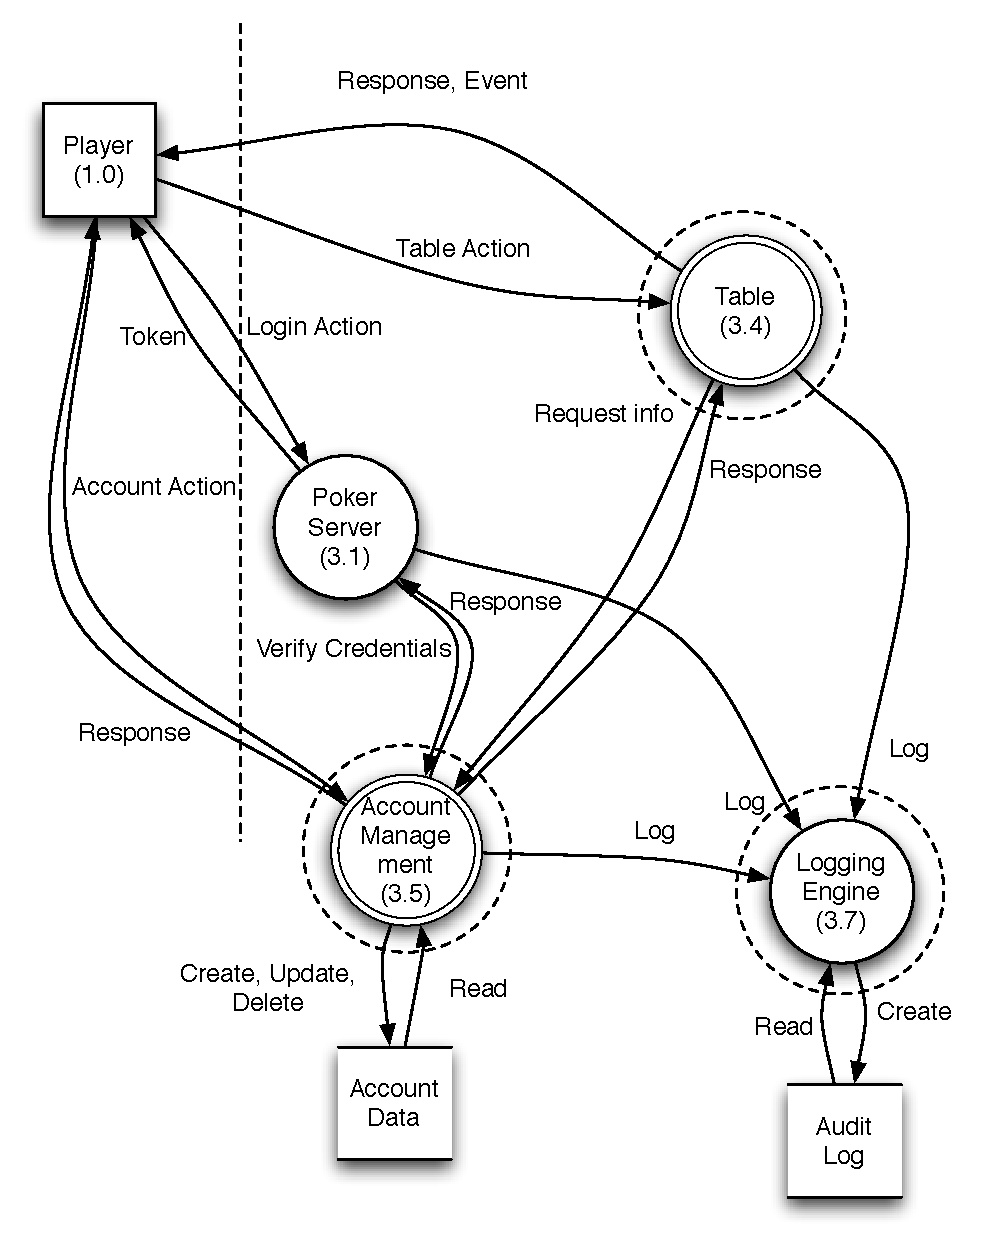
\includegraphics[scale=0.8]{dfd_level_0_player_simplified}
  \end{center}
  \caption{DFD Level-0 - only player - simplified}\label{fig:dfd_level_0_player_simplified}
\end{figure}
\begin{figure}[h]
  \begin{center}
    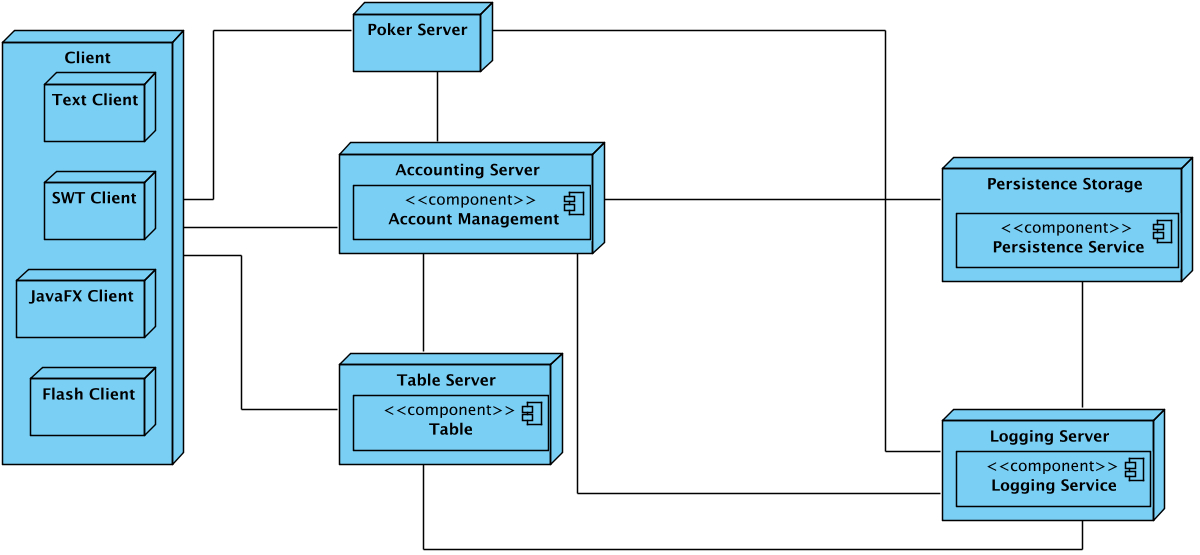
\includegraphics[angle=90,scale=0.65]{deployment_simplified.png}
  \end{center}
  \caption{Deployment View - simplified}\label{fig: deployment_simplified}
\end{figure}

\section{Security Objectives}
\label{MUCLabels}

\subsection{Authentication (26 MUCs)}
\begin{enumerate}
\item Spoofing a player
\item Repudiation of a player
\item Spoofing the poker server
\item Tampering with the poker server
\item Repudiation of the poker server
\item Information disclosure at the poker server
\item Elevation of privilege at the poker server
\item Spoofing a table
\item Tampering with a table
\item Repudiation of a table 
\item Information disclosure at a table 
\item Elevation of Privilege at the table
\item Spoofing the account management system
\item Tampering with the account management system
\item Repudiation of using the account management system
\item Information disclosure of the account management system
\item Elevation of Privilege at the account management system
\item Spoofing the logging engine
\item Tampering with the logging engine 
\item Repudiation of using the logging engine
\item Information disclosure of the logging engine 
\item Elevation of Privilege at the logging engine
\item Tampering with the audit log
\item Information disclosure of the audit log
\item Tampering with account data
\item Information disclosure of account data 
\end{enumerate}

\subsection{Authorization (21 MUCs)}
\begin{enumerate}
\item Repudiation of a player
\item Tampering with the poker server
\item Repudiation of the poker server
\item Information disclosure at the poker server
\item Elevation of privilege at the poker server
\item Tampering with a table
\item Repudiation of a table 
\item Information disclosure at a table
\item Elevation of Privilege at the table
\item Tampering with the account management system
\item Repudiation of the account management system
\item Information disclosure of the account management system
\item Elevation of Privilege at the account management system 
\item Tampering with the logging engine 
\item Repudiation of the logging engine 
\item Information disclosure of the logging engine 
\item Elevation of Privilege at the logging engine
\item Tampering with the audit log
\item Information disclosure of the audit log
\item Tampering with account data
\item Information disclosure of account data 
\end{enumerate}

\subsection{Application Integrity (12 MUCs)}
\begin{enumerate}
\item Tampering with the poker server
\item Information disclosure at the poker server
\item Elevation of privilege at the poker server
\item Tampering with a table
\item Information disclosure at a table 
\item Elevation of Privilege at the table
\item Tampering with the account management system
\item Information disclosure of the account management system
\item Elevation of Privilege at the account management system 
\item Tampering with the logging engine 
\item Information disclosure of the logging engine 
\item Elevation of Privilege at the logging engine
\end{enumerate}

\subsection{Availability (10 MUCs)}
\begin{enumerate}
\item Denial of Service against the poker server
\item Denial of Service against a table 
\item Denial of Service against the account management system
\item Denial of Service against the logging engine
\item Denial of Service against the audit log
\item Denial of Service against account data
\item Denial of Service of token requests 
\item Denial of Service of tokens 
\item Denial of Service of actions
\item Denial of Service of logging requests
\end{enumerate}

\subsection{Non-repudiation (6 MUCs)}
\begin{enumerate}
\item Repudiation of a player
\item Repudiation of the poker server
\item Repudiation of a table
\item Repudiation of the account management system
\item Repudiation of the logging engine 
\item Repudiation of the audit log
\end{enumerate}

\subsection{Transmission Integrity (5 MUCs)}
\begin{enumerate}
\item Tampering with token requests
\item Tampering with tokens
\item Tampering with actions
\item Tampering with responses and events 
\item Tampering with logging requests 
\end{enumerate}

\subsection{Transmission Confidentiality (5 MUCs)}
\begin{enumerate}
\item Information Disclosure of token requests
\item Information Disclosure of tokens
\item Information Disclosure of actions
\item Information Disclosure of responses and events
\item Information Disclosure of logging requests 
\end{enumerate}

\subsection{Auditing (4 MUCs)}
\begin{enumerate}
\item Repudiation of a player
\item Repudiation of the poker server
\item Repudiation of a table
\item Repudiation of the account management system
\end{enumerate}

\subsection{Storage Integrity (2 MUCs)}
\begin{enumerate}
\item Tampering with the audit log
\item Tampering with account data
\end{enumerate}

\subsection{Storage Confidentiality (2 MUCs)}
\begin{enumerate}
\item Information disclosure of the audit log
\item Information disclosure of account data 
\end{enumerate}

\subsection{Application Confidentiality}
Application Confidentiality is not applicable since the code is open source.

\chapter{Securing the architecture}

\section{Quality trade-off labels}
\label{labels}
By analyzing the business goals, we constructed the following ordered list of quality trade-off labels:
\begin{enumerate}
\item Usability: the online casino has to be as easy to use as possible.
\item Confidentiality: it is of the abmost importance that certain information like the cards of a player, remains
confidential.
\item Integrity: no one should be able to compromise the integrity of the application or it's data.
\item Accountability: no player may be able to repudiate any bets or other actions.
\item Manageability: the application must be easy to manage by an admin.
\item Cost: the cost of the application should be reasonable to low, so profit will remain solid.
\item Performance: performance being the possible amount of games played simultaneously, is important because it
determines the maximum profit.
\item Maintainability: the application should be easy to maintain.
\end{enumerate}
These labels will be used to guide the selection of security patterns in the next section.
\section{Detailed description of the followed steps}
We will use the security patterns and methodology described in \cite{yskout} to select the appropriate patterns
for this application.

\subsection{Analysis Phase}
The analysis phase consists of eliciting the security requirements and annotating each 
security requirement with the security object it belongs to. The security requirements have been elicited by the misuse cases
in secton \ref{MisUseCases}. The annotations to indicate for each misuse case to which security objective it belongs are given in section \ref{MUCLabels}. This is very important, since the succes of the selected methodology heavily depends 
on this list of security requirements.

\subsection{Architecture Phase}
As stated in \cite[p13]{yskout}, the architecture of the system is designed using Attribute-Driven Design or ADD,
meaning it is created based on the non-functional requirements of the application and their relative importance.
Therefore a prioritized list of quality attributes, inspired by the business goals, was formulated under 
\ref{labels}. Then we iterate over the selection of architectural patterns, as it is stated by the methodology.

\subsubsection{Patterns already present}
There are some security patterns that are already present in the architecture:
\begin{itemize}
\item Credential Tokenizer: The poker server is in a certain way a credential tokenizer: it provides a token to a 
player that the player can use to authenticate himself with the other processes.
\item Secure Service Facade: Every process has it's own facade where all the needed
security checks happen.
\item Secure Logger: the Logging Engine performs the tasks of a Secure Logger.
\end{itemize}

\subsubsection{Authentication}
The authentication requirement covers the most misuse cases so it is selected as the first requirement to cover.

The following patterns address authentication at the architectural level:
\begin{itemize}
\item Authentication Enforcer
\item Credential Tokenizer
\item Security Association
\item Secure Service Facade
\item Session
\item Single Access Point
\end{itemize}

Credential Tokenizer and Secure Service Facade are already present in the architecture.

Since these two patterns do not sufficiently cover Authentication, we continue with the set of patterns that aren't
present yet: Authentication Enforcer, Security Association, Session and Single Access Point.

There are no patterns in this list that conflict with any existing patterns.
Next, we screen the short descriptions of the selected patterns to see if they are applicable. 
\begin{itemize}
\item Security Association appears to be missing from the list and is therefore discarded. 
\item Session won't be selected, because there is too 
little shared state between the different processes; the state is almost only shared within a process.                                                                               \end{itemize}

The other patterns seem applicable.

Authentication Enforcer has as labels +Maintainability, +Manageability, +Auditability, -Anonymity, +Privacy, 
+Accountability, +Portability and benefits from Secure Pipe and Secure Service Facade and has as alternative
Container Managed Security.

Single Access Point has as labels +Manageability and has no relations with other patterns.

Clearly Authentication Enforcer is the best choice here: it's labels match more with the quality trade-off labels
than Single Access Point, and it benefits from the Secure Service Facade pattern that already exist in the architecture
.Single Access Point would also lead to a too centralised architecture.Container Managed 
Security is a system pattern and will later be considered as an
alternative for Authentication Enforcer.

So the Authentication Enforcer pattern is selected and instantiated to deal with the Authentication 
requirement. //TODO

We can now mark the Authentication requirement as resolved.

\subsubsection{Authorization}
For Authorization, we follow the same steps as with Authentication.

The following patterns address authorization at the architectural level:
\begin{itemize}
\item Authorization Enforcer
\item Controlled Object Monitor
\item Full View With Errors
\item Limited View
\item Secure Service Facade
\item Single Access Point
\end{itemize}

Secure Service Facade is already present in the architecture. Single Access Point was already considered under 
Authentication.

So the list of selected candidates is Authorization Enforcer, Controlled Object Monitor, Full View With Errors
and Limited View.

There are no patterns in this list that conflict with any existing patterns.
Next, we screen the short descriptions of the selected patterns to see if they are applicable. Controlled Object
Monitor isn't applicable because there are few shared objects between processes so there is little need to monitor
and intercept acces requests from different processes to objects. The other patterns seem applicable.

Authorization Enforcer has as labels +Maintainability, +Manageability, +Auditability, +Accountability and
+Portability , and benefits from Authentication Enforcer and Secure Service Facade and has as alternative
Container Managed Security.

Full View With Errors has as labels +Maintainability, -Usability and conflicts with Limited View and has as
alternative Limited View.

Limited View has as labels +Usability and conflicts with Full View With Errors and has as alternative Full View 
With Errors.

Authorization Enforcer will be selected, because it has many + labels that match the quality trade-off labels and
it benefits from already instantiated patterns such as Authentication Enforcer and Secure Service Facade. It's
alternative, Container Managed Security, is a system pattern and will be consider later. Maybe we will have to
backtrack over the choices we made if the alternative appears to be a better choice.

Both Limited View and Full View with Errors will be selected, but for different parts so there is no conflict.
Limited View will be used for the client side, because Usability for the clients is a major issue. Full View with
Errors will be used for the server api.

So the Authorization Enforcer, Limited View and Full View With Errors are selected and instantiated 
to deal with the Authorization requirement.

We can now consider the Authorization requirement as resolved.
\subsubsection{Application Integrity}
The following patterns address application integrity at the architectural level:
\begin{itemize}
\item Checkpointed System
\item Comparator-Checked Fault-Tolerant System
\end{itemize}

There are no patterns in this list that conflict with any existing patterns.
Next, we screen the short descriptions of the selected patterns to see if they are applicable. Both patterns seem
applicable.

Checkpointed System has as labels +Dependability, -Performance and -Cost , and benefits from Comparator Checked
 Fault Tolerant System and impairs Audit Interceptor.

Comparator-Checked Fault-Tolerant System has as labels -Cost, -Performance, +Dependability and impairs Audit
Interceptor and has as alternative Output Guard and benefits from Checkpointed System.

Checkpointed System will be selected, even though it has a negative influence on both the Cost and the Performance,
because there must be a way to recover from a crash of a critical process such as Cashier. So the Cashier process
will be checkpointed: the cashier will reserve the money used in bets of a deal. When the deal ends, the table 
will tell the cashier the money can be really transfered. If for some reason, the table fails and the deal is 
cancelled, the money used in that deal will go back to it's owners.

Comparator-Checked Fault-Tolerant System won't be selected because it is considered overkill, and has too little
advantages compared to it's disadvantages.

So the Checkpointed System pattern is selected and instantiated to deal with the Application Integrity requirement.
We can now consider the Application Integrity requirement as resolved.
\subsubsection{Accountability}
\begin{itemize}
\item Secure Logger
\end{itemize}
Secure Logger is already present in the architecture, the Accountability requirement is considered as solved.
\subsubsection{Data Integrity}
The following patterns address application integrity at the architectural level:
\begin{itemize}
\item Session
\item Secure Access Layer
\item Secure Pipe
\end{itemize}

There are no patterns in this list that conflict with any existing patterns.
Next, we screen the short descriptions of the selected patterns to see if they are applicable. Both patterns seem
applicable.

Secure Access Layer has as labels +Maintainability and +Portability, and has no relations with other patterns.

Secure Pipe has no labels in the list, but we believe it should have +Confidentiality and +Integrity. The pattern
benefits from Secure Association (which by the way is not included in the list, see \ref{criticism}.

Secure Access Layer will be selected because it has only positive labels and has no relation with other patterns.
Secure Pipe will be selected because confidentiality and integrity are considered important quality labels.

So Secure Access Layer and Secure Pipe are selected and instantiated to deal with the Data Integrityrequirement.

We can now consider the Data Integrity requirement as resolved.


\subsubsection{Availability}
\begin{itemize}
\item Checkpointed System
\item Load Balancer
\item Replicated System
\end{itemize}
\subsection{Design Phase}
We don't consider design phase and patterns because it isn't part of the assignment and it would be too
low level.
\subsection{System Phase}
As stated in \cite[p13]{yskout}, the architecture of the system is designed using ADD or Attribute-Driven Design,
meaning it is created based on the non-functional requirements of the application and their relative importance.
Therefore a prioritized list of quality attributes, inspired by the business goals, was formulated under 
\ref{labels}. Then we iterate over the selection of architectural patterns, as it is stated by the methodology.

\subsubsection{Authentication}
The authentication requirement covers the most misuse cases so it is selected as the first requirement to cover.
The following patterns address authentication at the architectural level:
\begin{itemize}
\item Container Managed Security
\end{itemize}

\subsubsection{Authorization}

\begin{itemize}
\item Application Firewall
\item Container Managed Security
\item Controlled Process Creator
\item Controlled Object Factory
\item Demilitarized Zone
\item Firewall
\end{itemize}

\subsubsection{Application Integrity}
No patterns

\subsubsection{Accountability}
\begin{itemize}
\item Audit Interceptor
\end{itemize}

\subsubsection{Data Integrity}
\begin{itemize}
\item Secure Message Router
\end{itemize}

\subsubsection{Availability}
No patterns
\subsection{Selected Patterns}
To summarize, here is the list of the selected patterns:
\begin{itemize}
\item Authentication Enforcer
\item Authorization Enforcer
\item Secure Pipe
\item Full View with Errors
\item Limited View
\item Application Firewall
\item Firewall
\item Checkpointed System
\item Audit Interceptor
\item Secure Access Layer
\item Load Balancer
\end{itemize}

\section{Criticism}
\label{criticism}
\begin{itemize}
\item The classification of the threat tree isn't very clear sometimes: e.g. you can tamper with the server process
to spoof the server and thus tampering with the data.
\item The threat three isn't complete; for instance there is nothing in it about spoofing by corruption of 
DNS records.
\item Some business use cases can't be covered with the list of security patterns in the given catalog
\item The list of labels is incomplete for some security patterns in the catalog: e.g. Secure Pipe should also have
the confidentiality-label.
\item Some patterns that are mentioned by other security patterns, aren't listed in the catalog: e.g. Secure Pipe 
benefits from Security Association, but the latter pattern isn't listed in the catalog. Input Guard also isn't
in the list.
\item Repudiaton of processes/data stores that are all internal to the system is very unclear. In the lectures it was said that this was, for instance, the casino denying that it did something. In \cite[p270]{1202957} however it is explained as an external entity tampering with the process/data store to be able to deny having done something. The difference with repudiaton of that external entity is unclear.
\end{itemize}
\section{Log}
\textbf{30-10-2008}
\begin{itemize}
\item We decided to only consider the RMI protocol as communication protocol for the poker application in this 
security analysis, and to not got into depth in the sockets or http protocol. For these protocols, a front-end is added to the architecture that delegates to the different processes also used by RMI.
\item Table communicates with Cashier instead of with Account Management process to obtain an amount of chips
of the main stack of a player and bring it to the table stack of that player.
\item For liability reasons, the log with game details must be made public after a game. This is reflected in some
business threats where a mis-actor might use this to profile certain players.
\item We decided to connect complex process in the Level 0 DFD directly to data stores so whe can apply STRIDE
at this level. Otherwise the number of misuse cases would explode.
\end{itemize}

\nocite{1202957}
\nocite{citeulike:174301}
\nocite{yskout}

\addcontentsline{toc}{chapter}{Bibliography}
\bibliography{oass2}

\end{document} 
